\graphicspath{{chapters/loadings/}}
\chapter{HCP and ADNI Loadings}\label{appendix:loadings}

This appendix builds upon the results presented in Chapter \ref{ch:als}, where we introduced a method to regularize CCA using structured priors on model weights, demonstrated with Human Connectome Project (HCP) and Alzheimer's Disease Neuroimaging Initiative (ADNI) data. In light of the insights gained from Chapter \ref{ch:loadings}, which examined the relationship between loadings and weights in CCA using simulated data, we revisit the HCP and ADNI results to further explore the interpretability of the models.


\section{Human Connectome Project (\acrshort{hcp}) Data}

\subsection{Brain Connectivity Weights and Loadings}

\begin{figure}
    \centering
    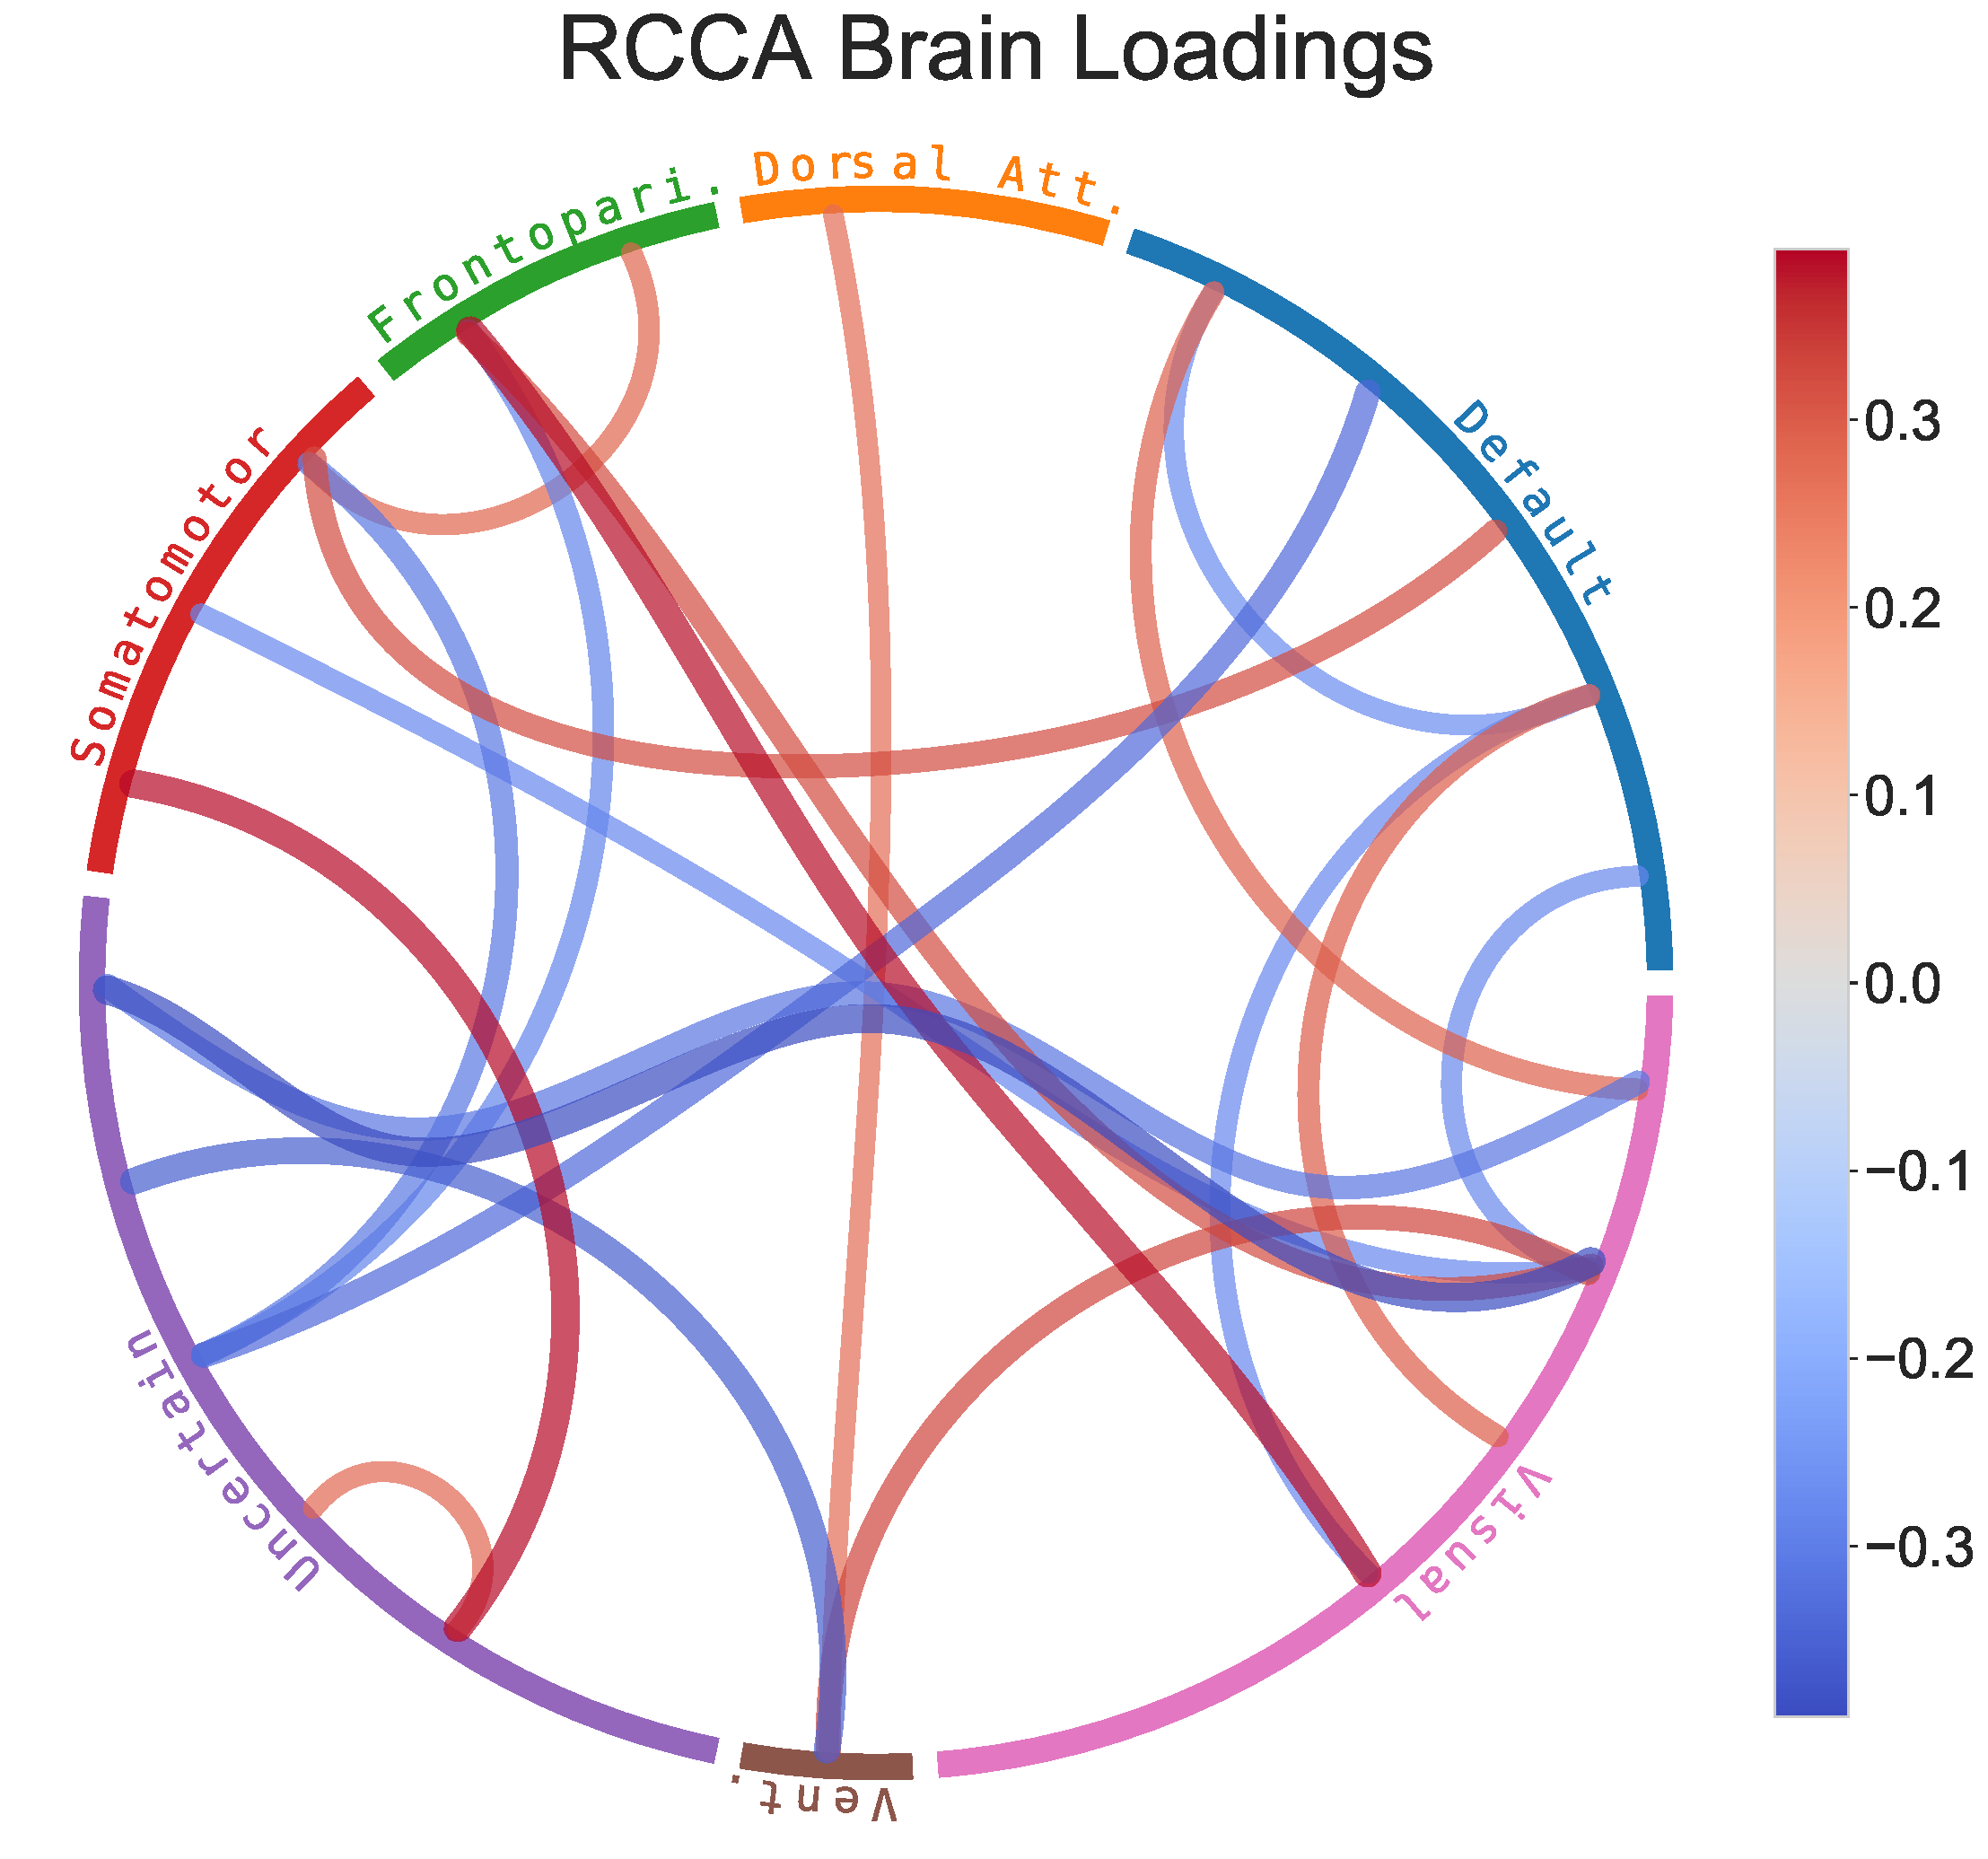
\includegraphics[width=0.49\linewidth]{figures/hcp/RCCA brain loadings}
    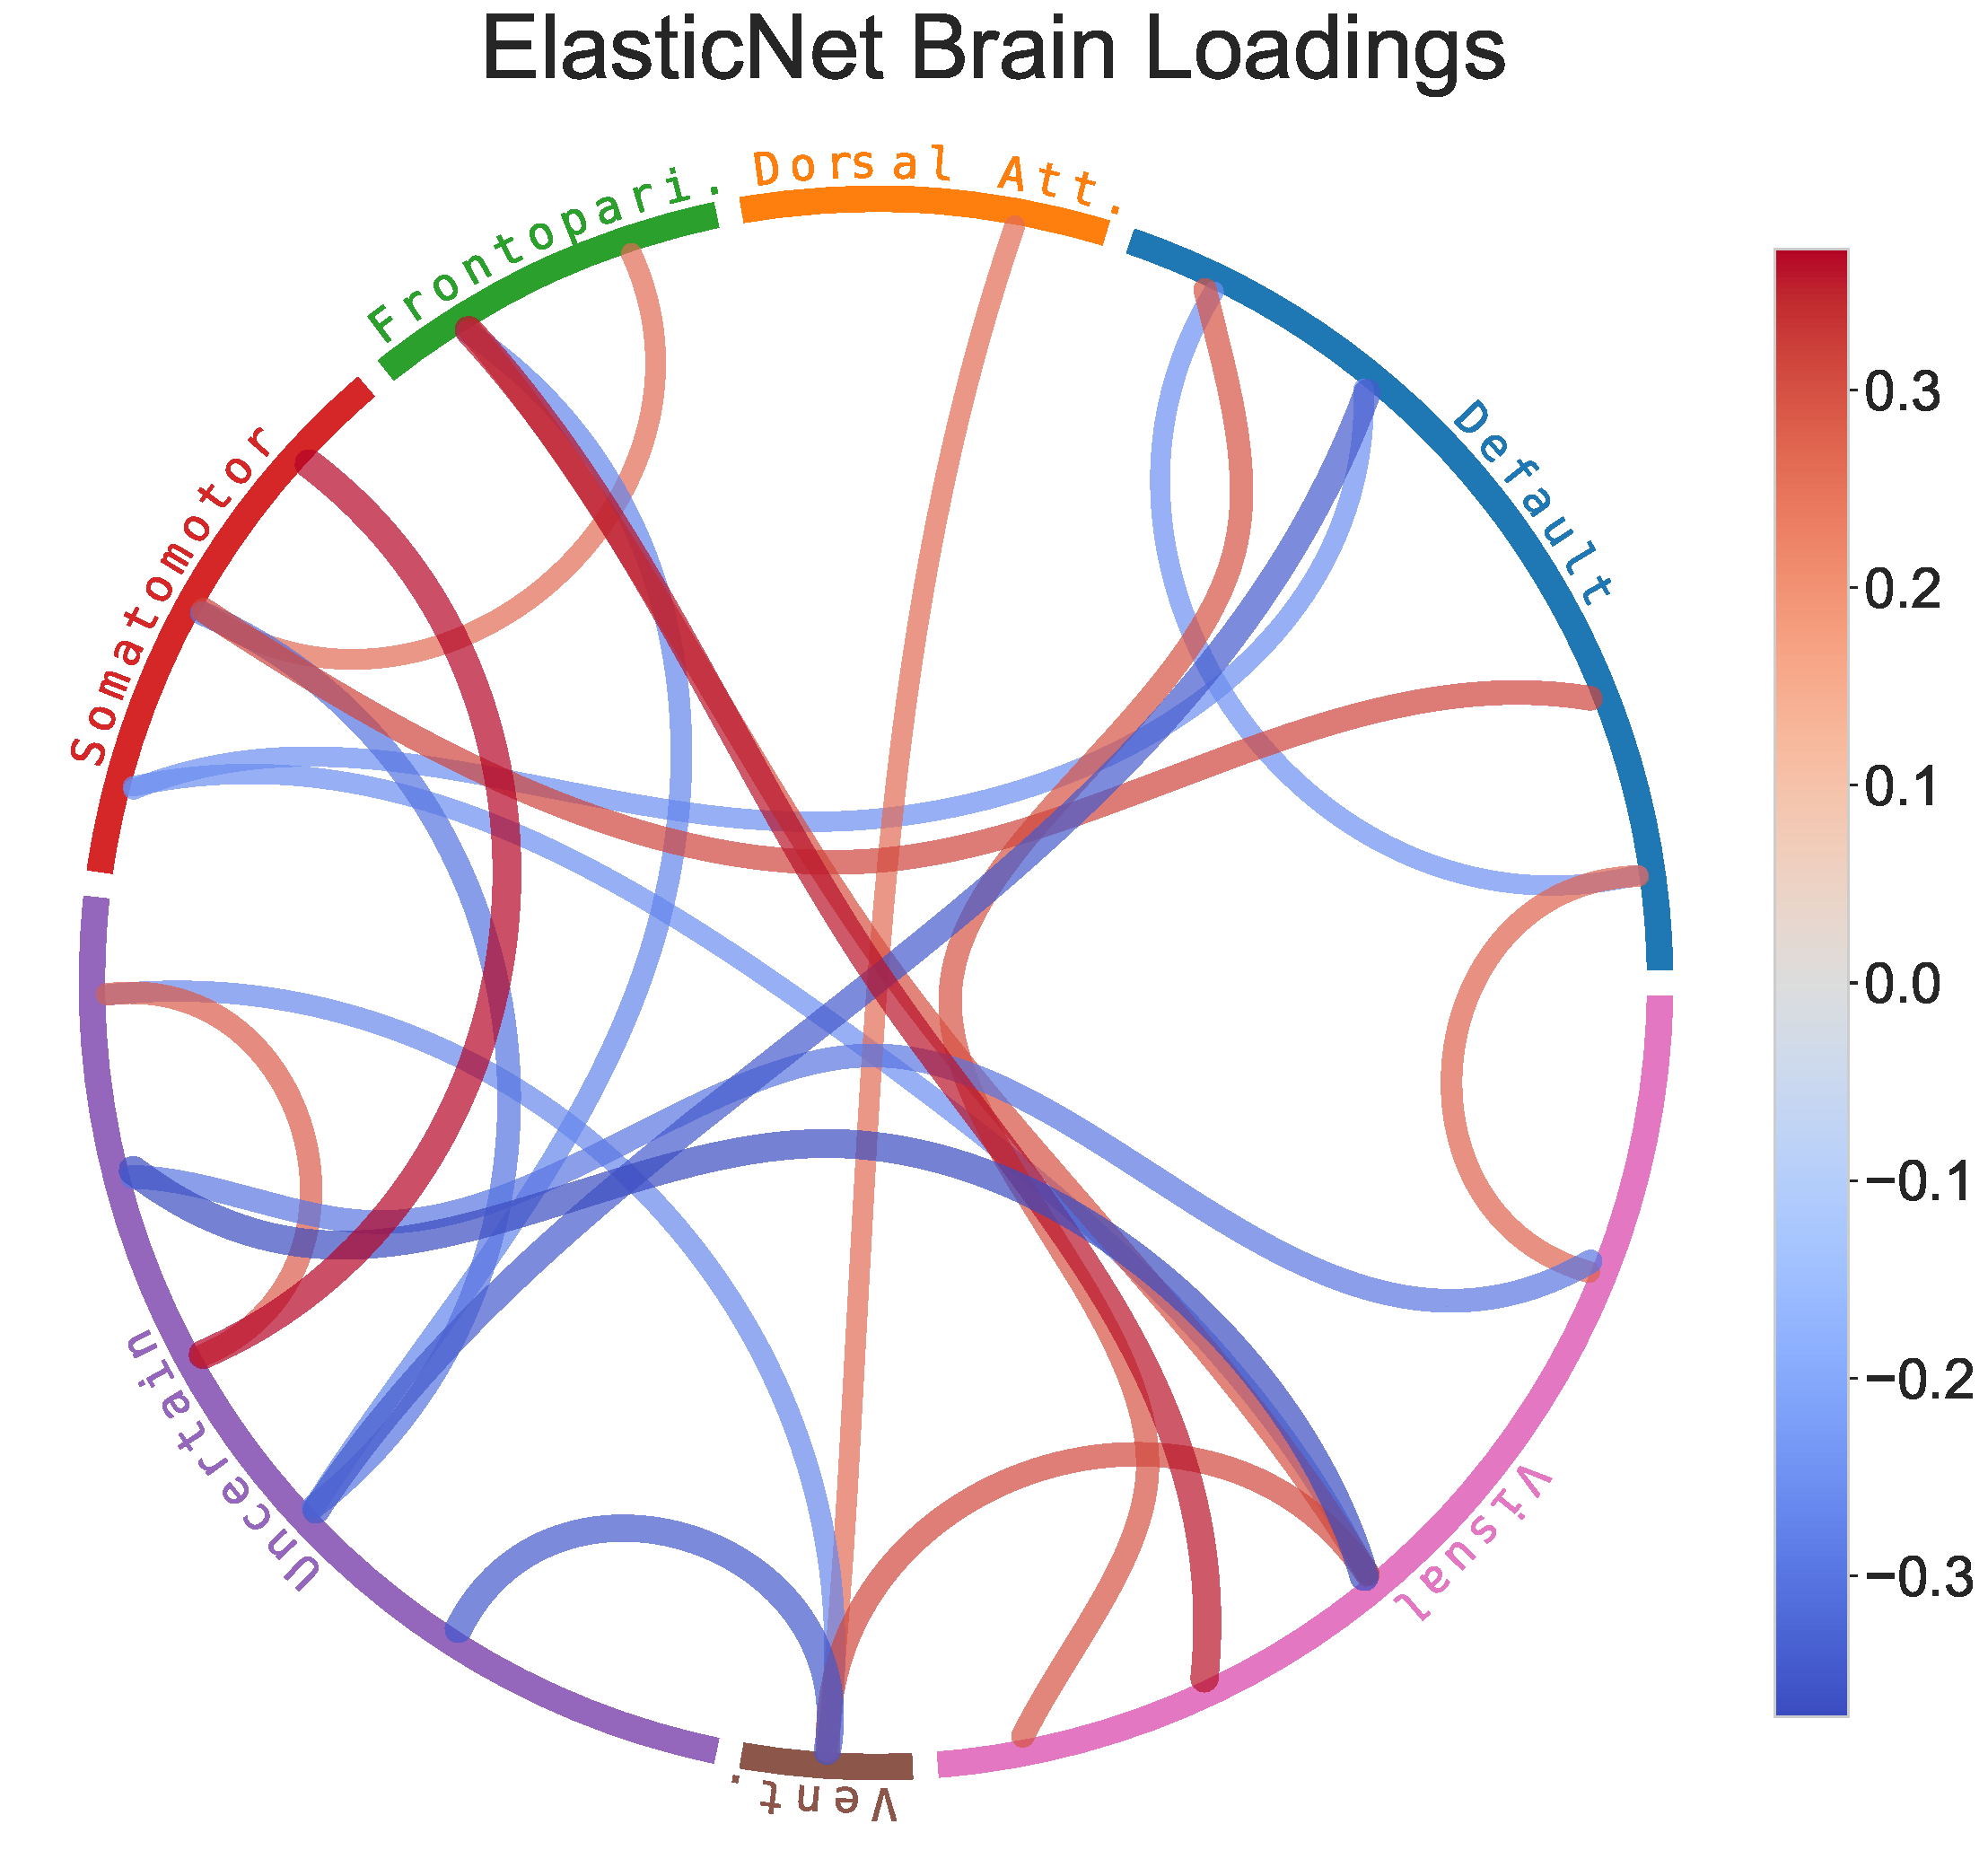
\includegraphics[width=0.49\linewidth]{figures/hcp/ElasticNet brain loadings}
    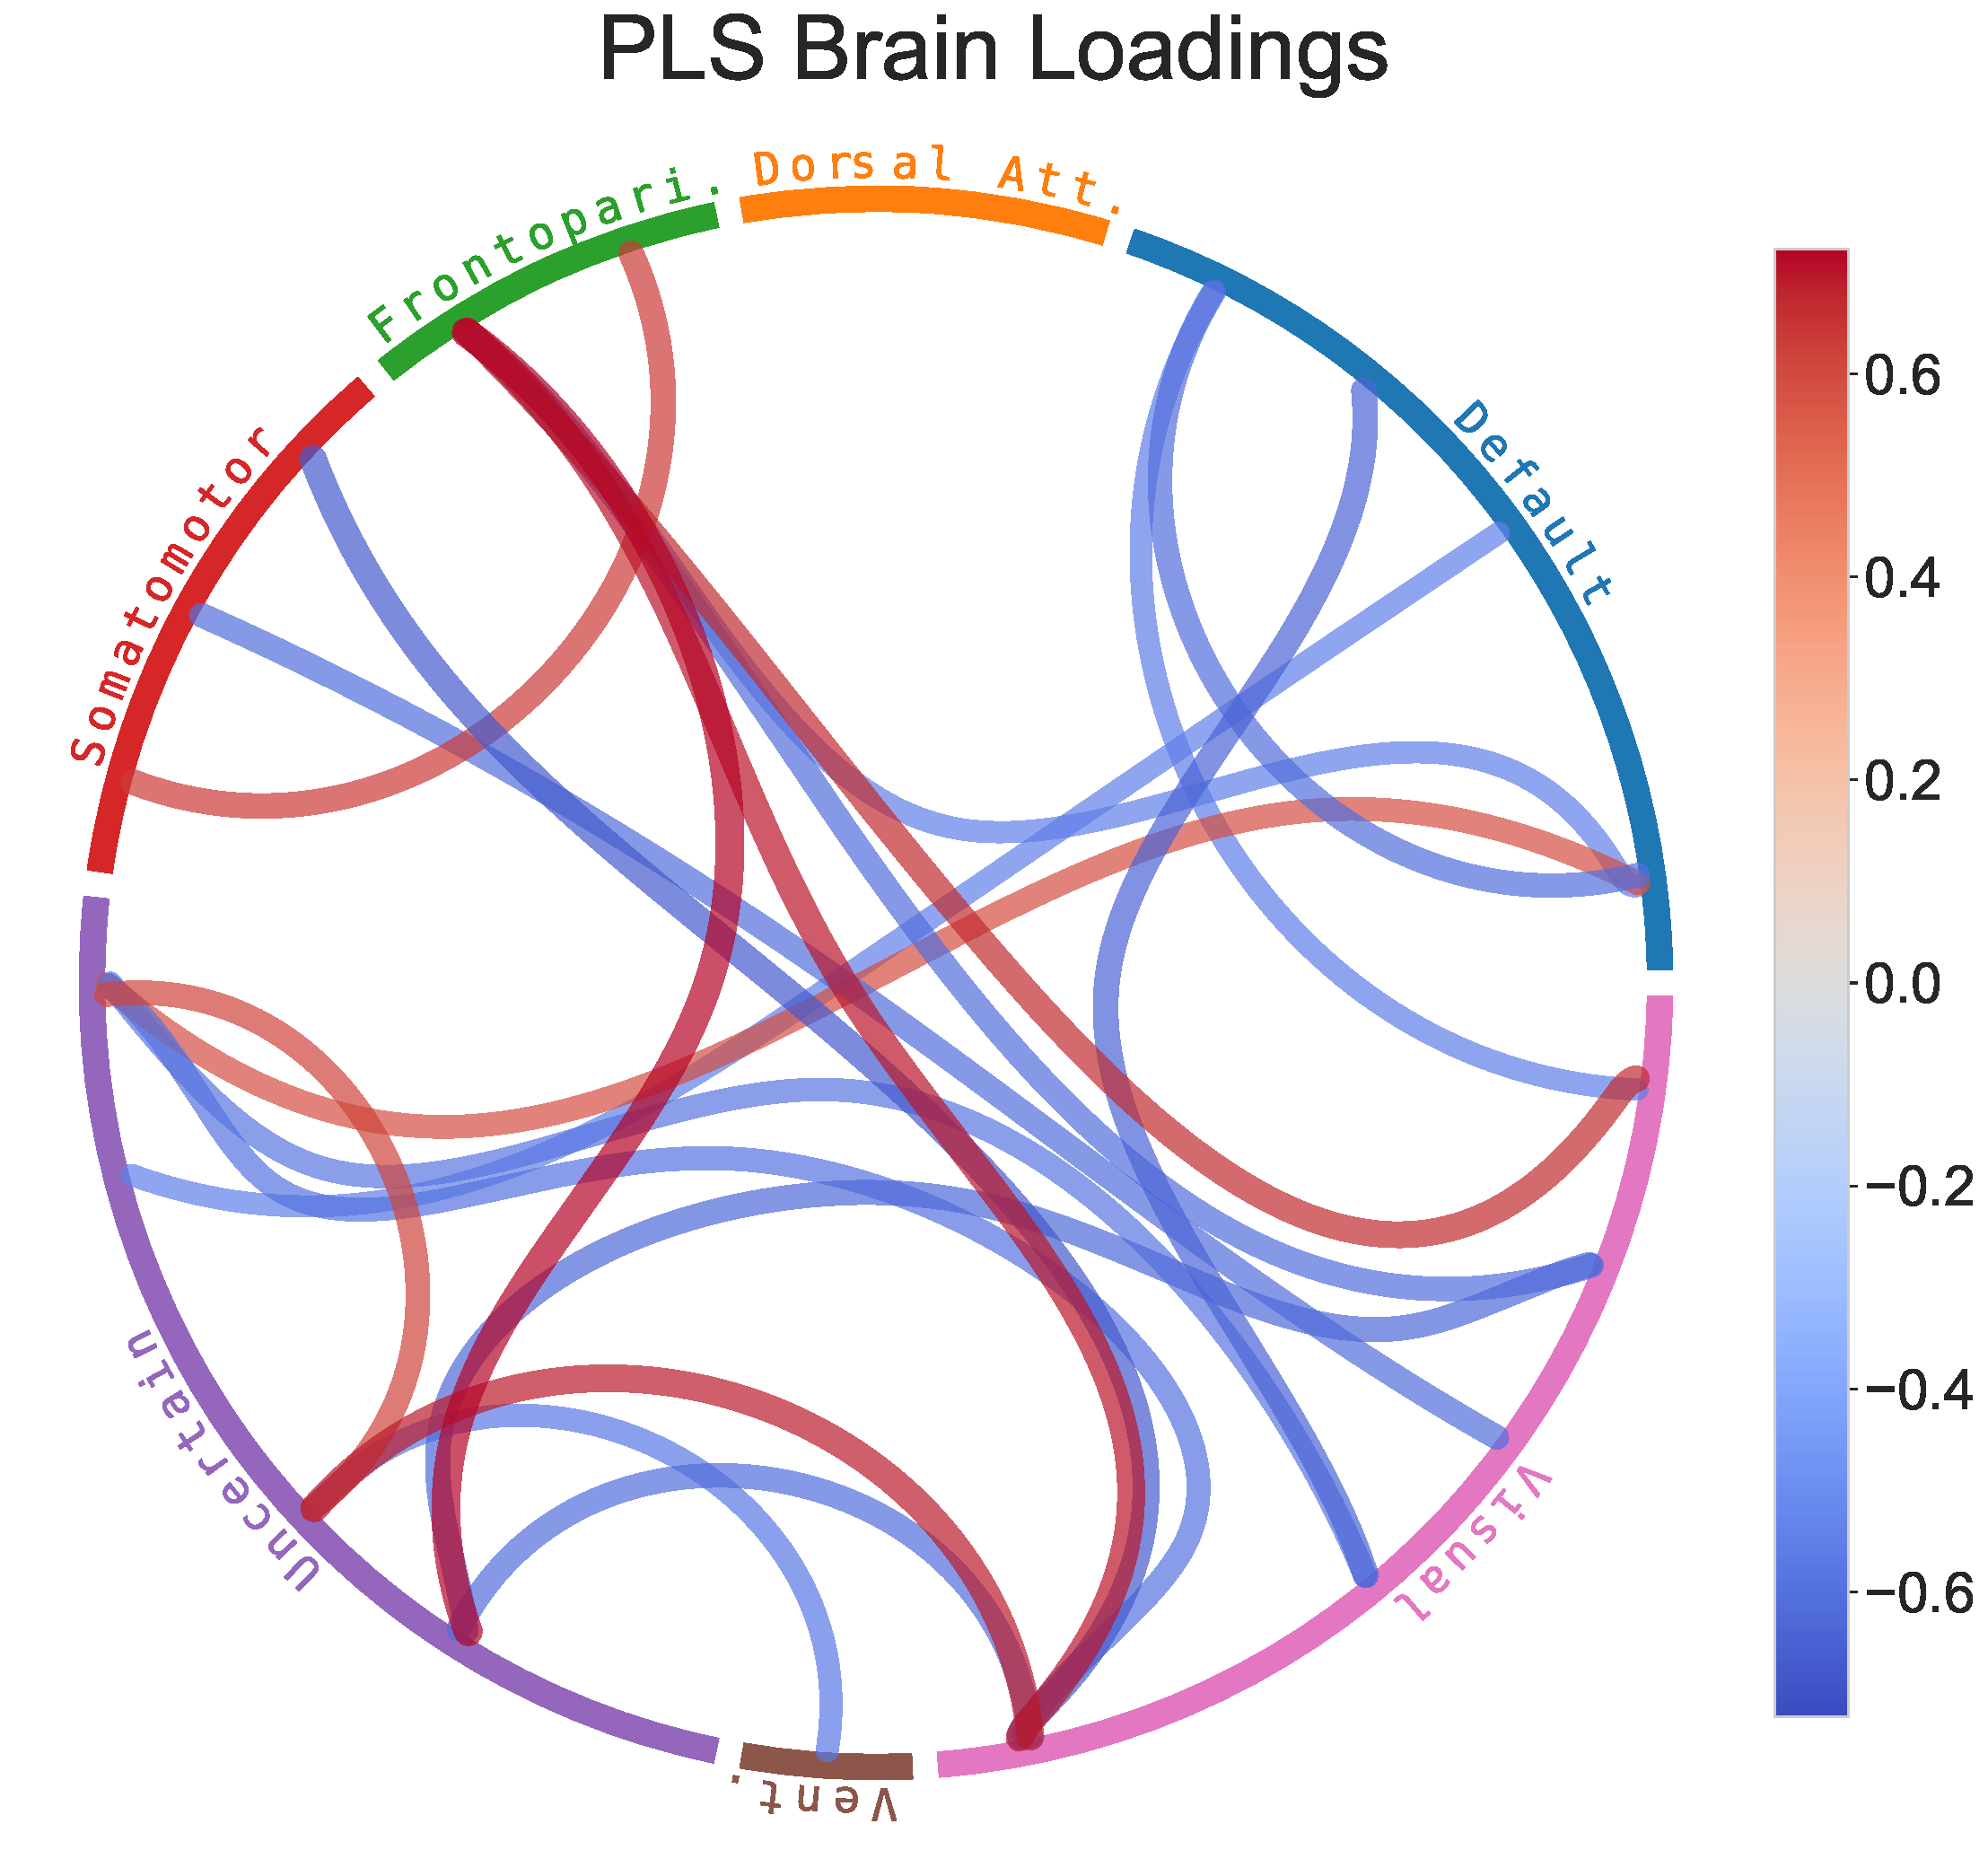
\includegraphics[width=0.49\linewidth]{figures/hcp/PLS brain loadings}
    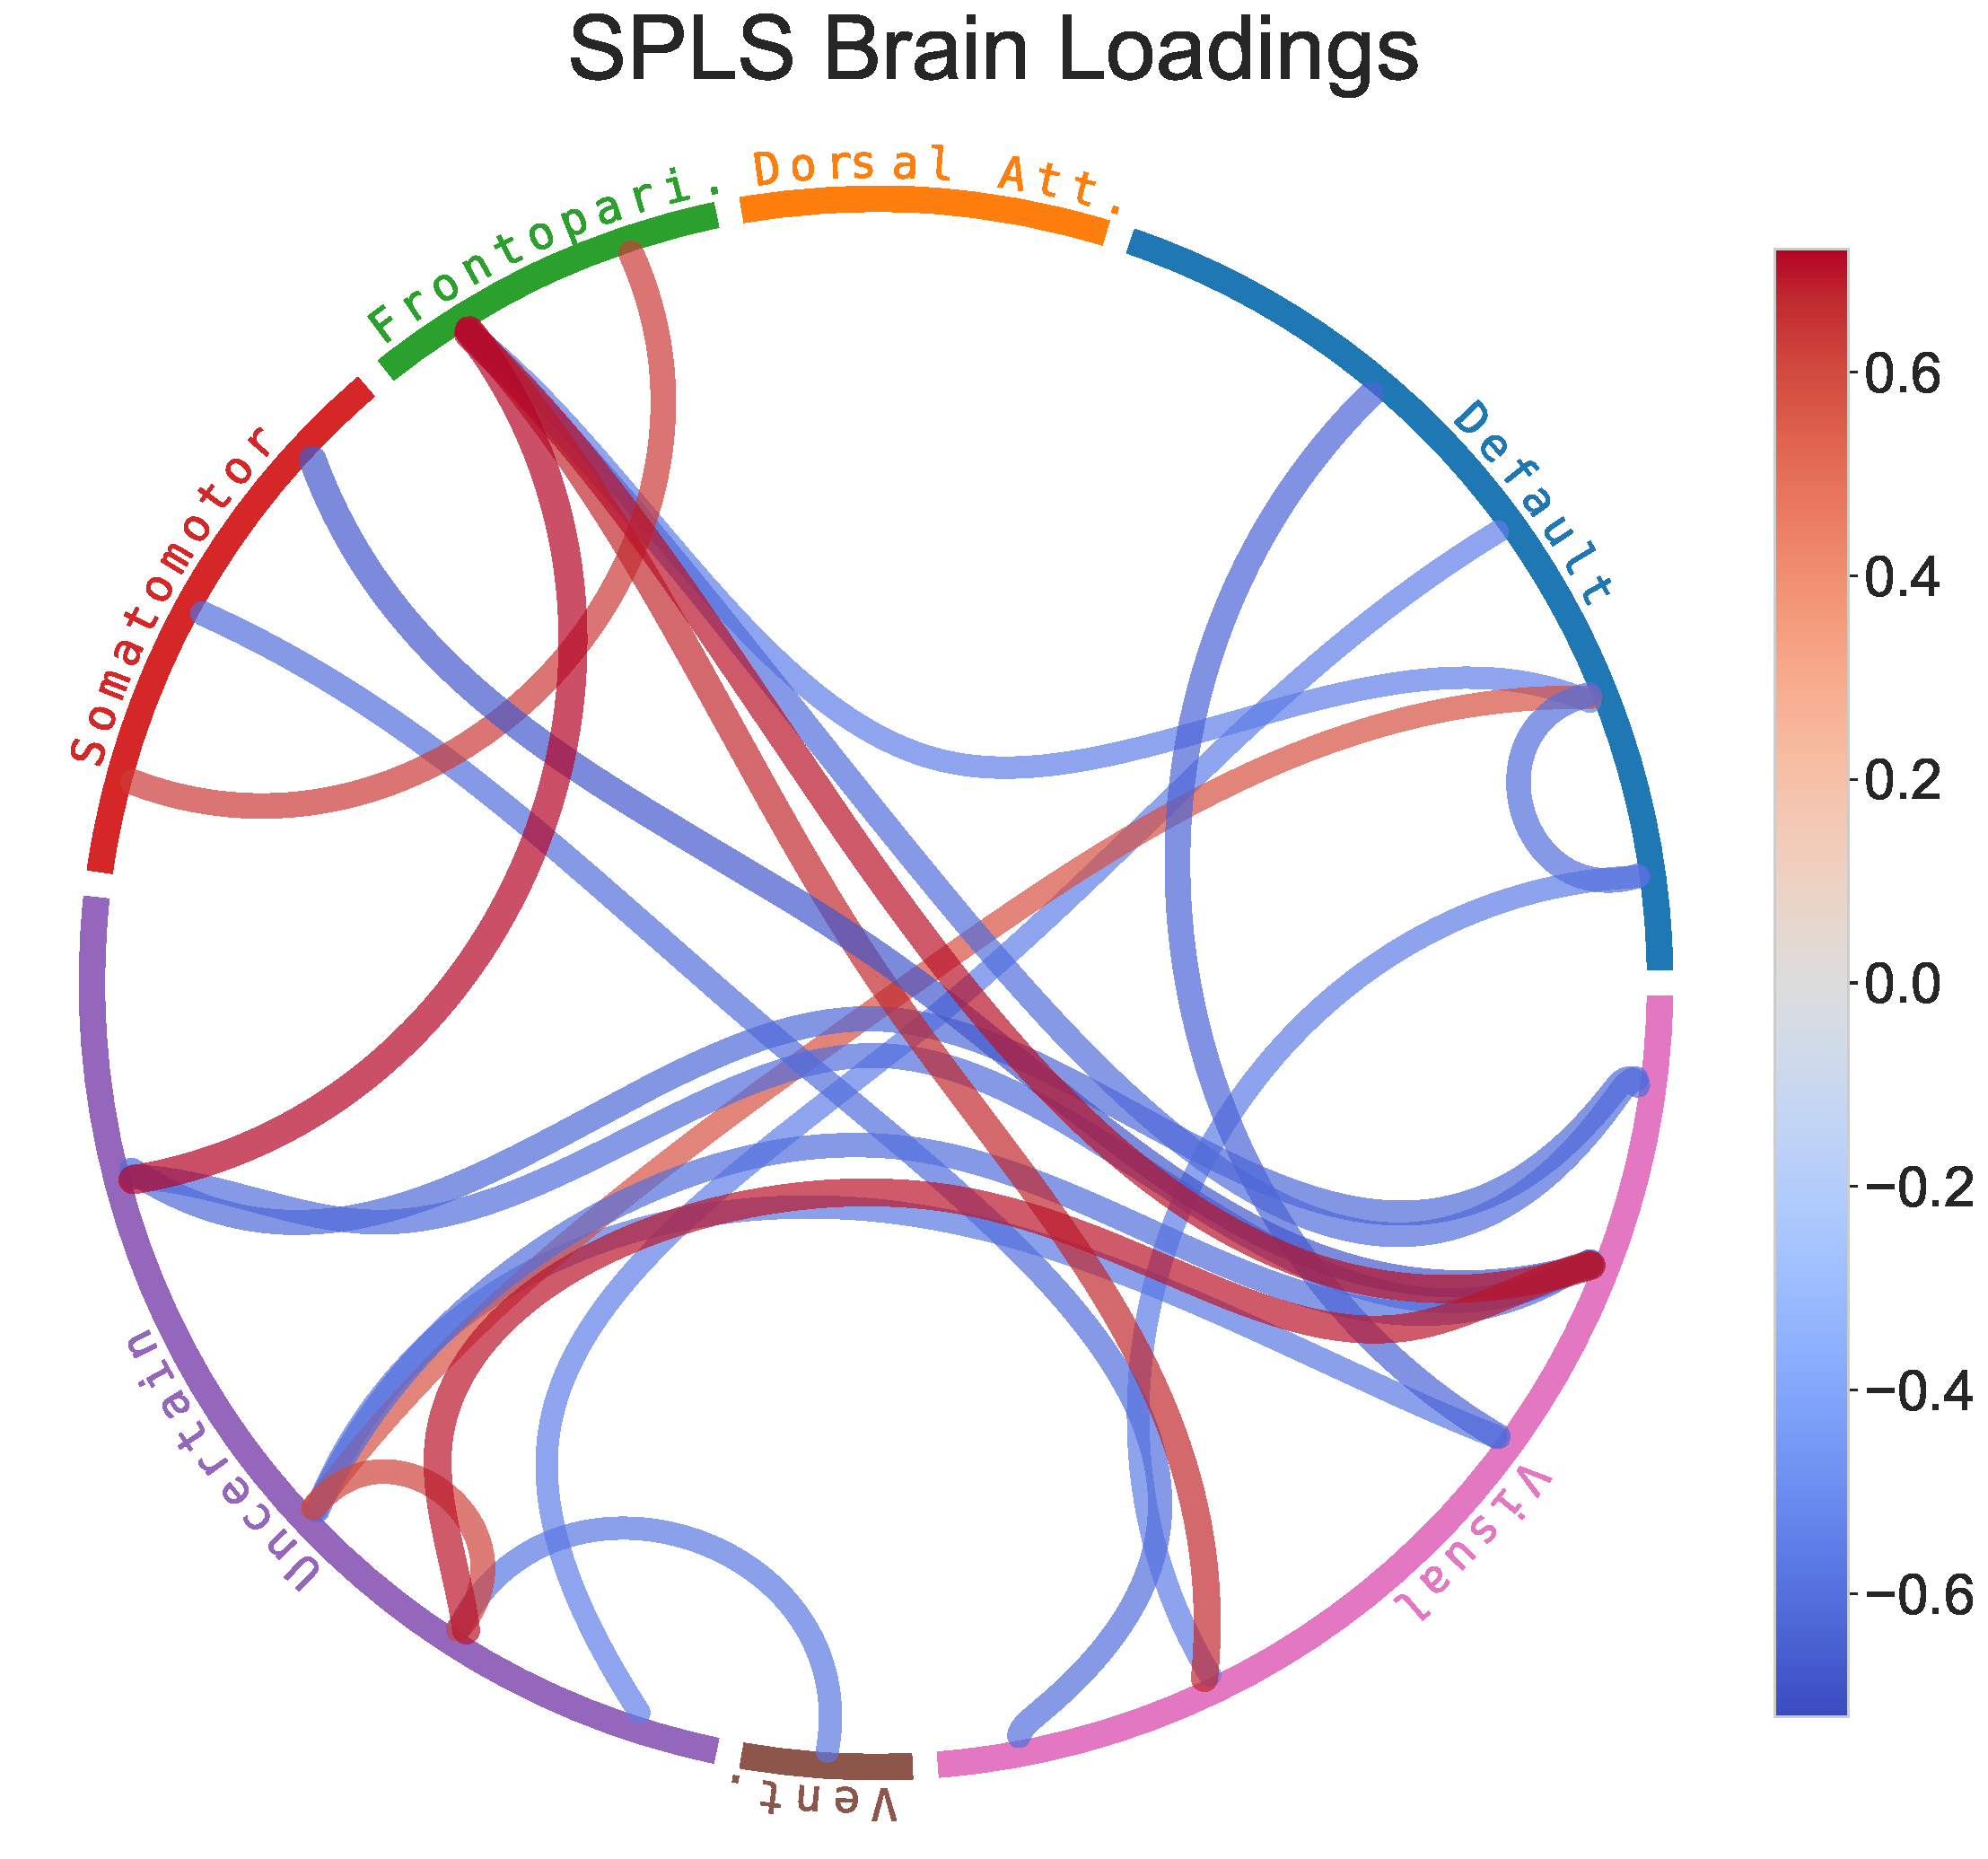
\includegraphics[width=0.49\linewidth]{figures/hcp/SPLS brain loadings}
    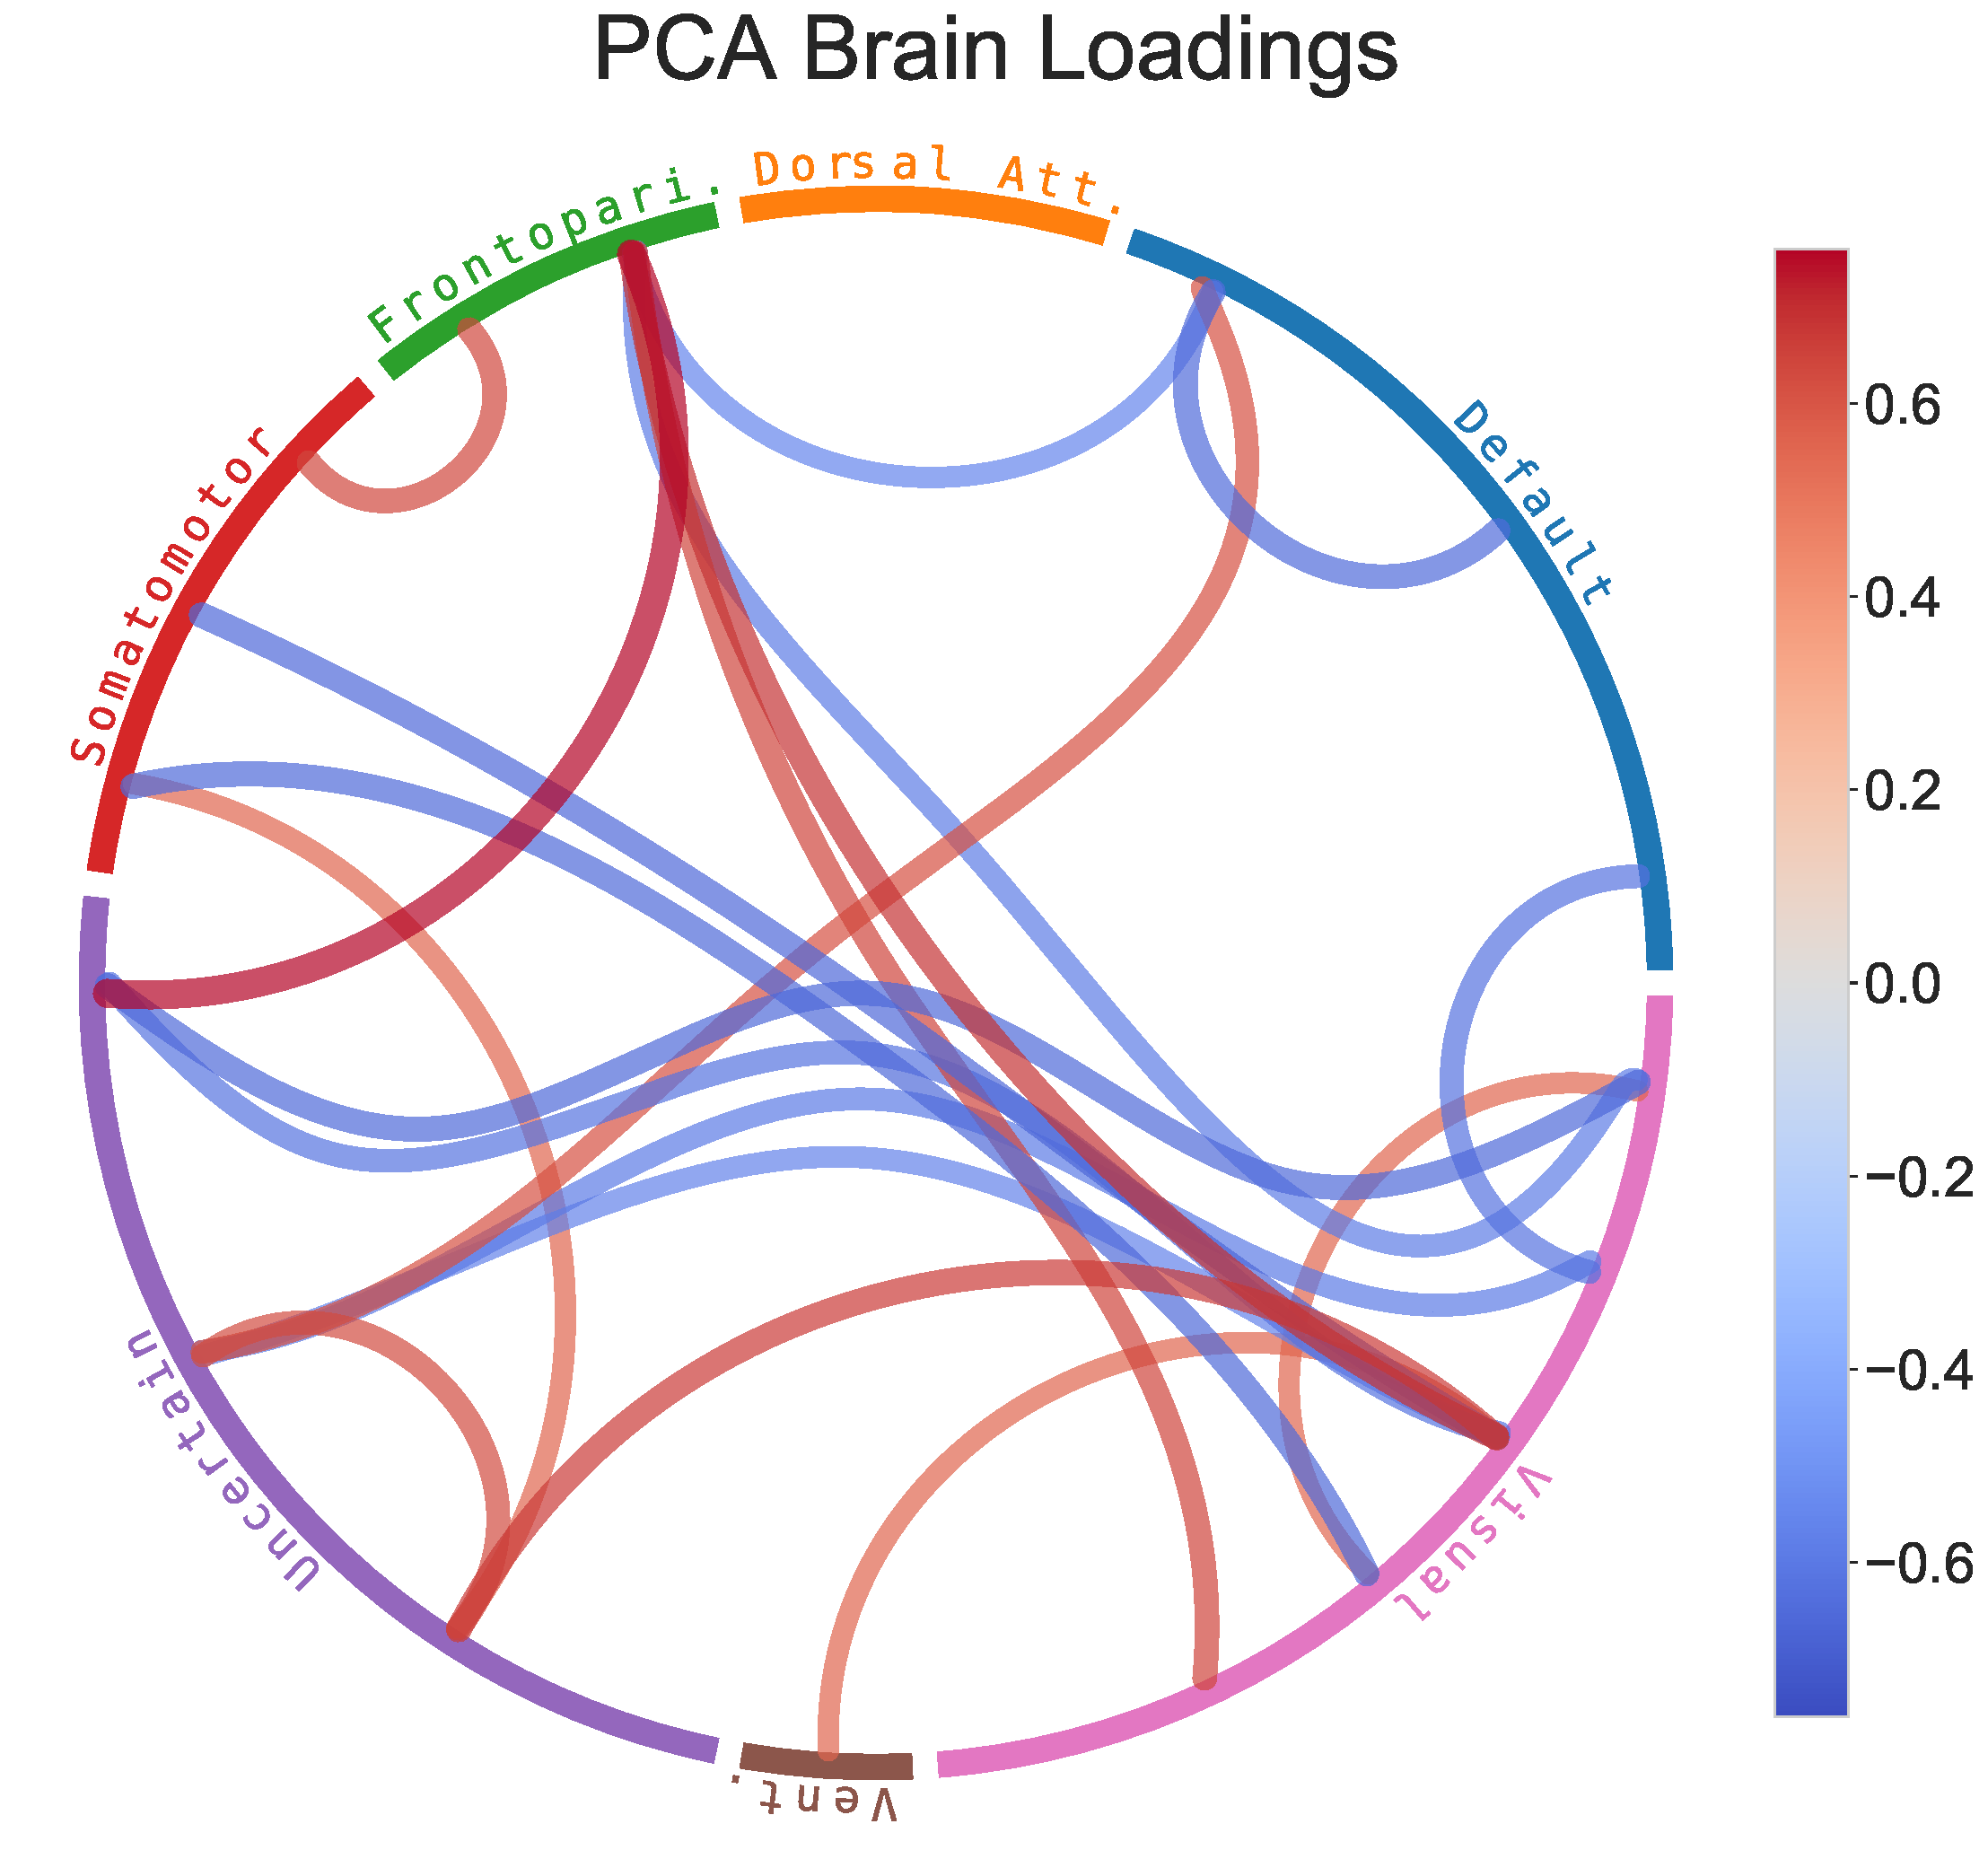
\includegraphics[width=0.49\linewidth]{figures/hcp/PCA brain loadings}
    \caption{Chord diagrams of the top 8 positive and negative brain \gls{loadings} for each model.}\label{fig:chord_loadings}
\end{figure}

\newpage


\section{Alzheimer's Disease Neuroimaging Initiative (\acrshort{adni}) Data}

\subsection{Brain Structure Weights and Loadings}

\begin{figure}
    \centering
    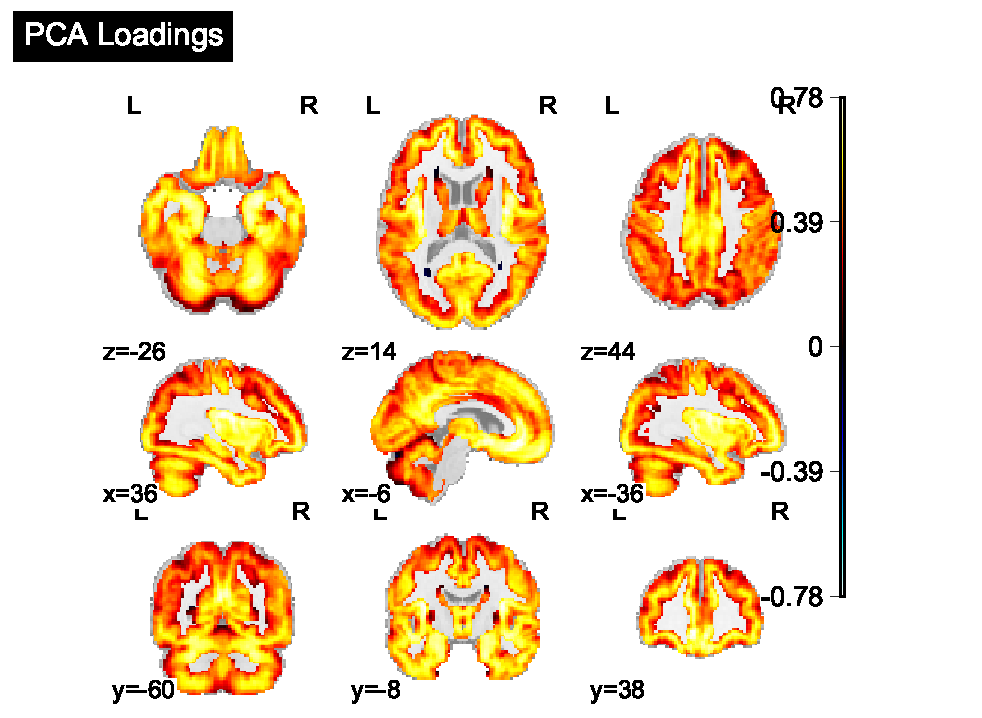
\includegraphics[width=0.45\linewidth]{figures/adni/PCA brain loadings mosaic}
    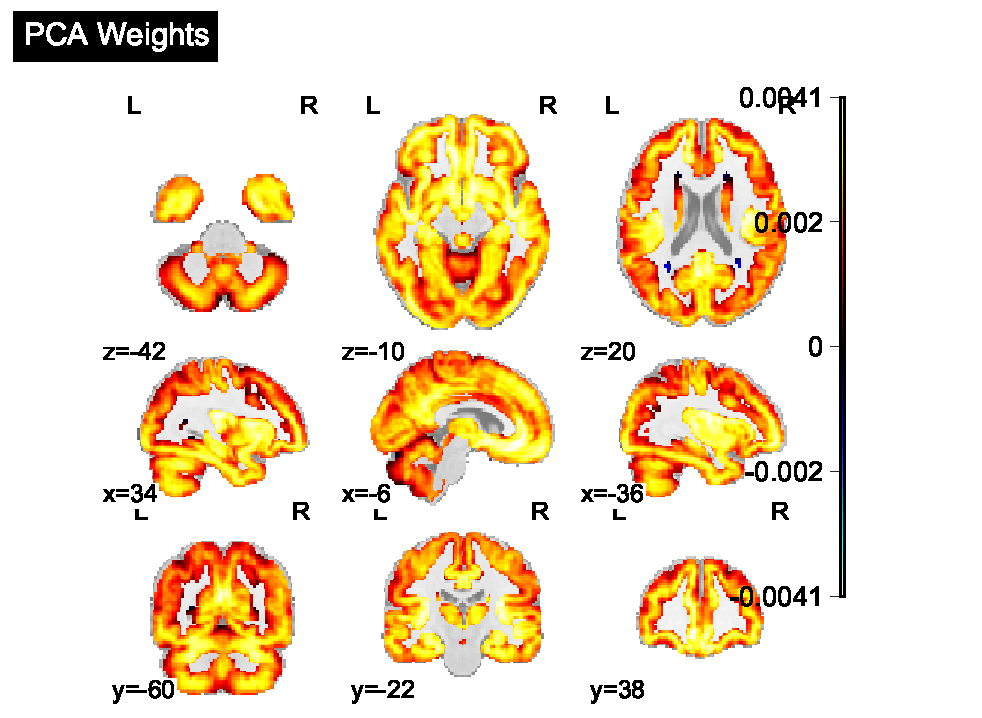
\includegraphics[width=0.45\linewidth]{figures/adni/PCA brain weights mosaic}
    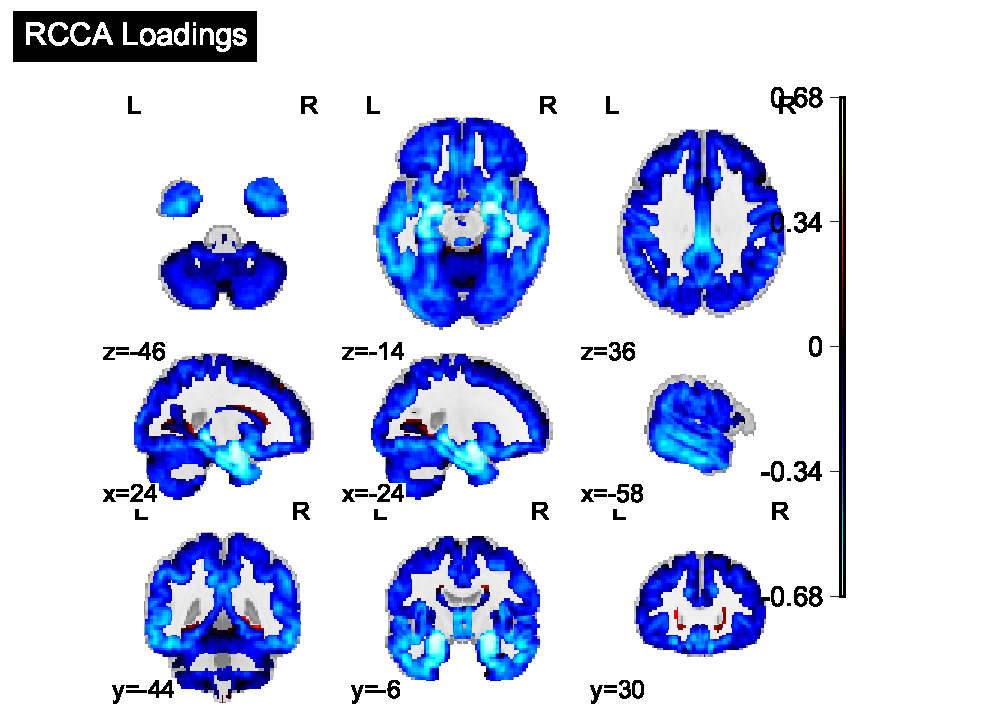
\includegraphics[width=0.45\linewidth]{figures/adni/RCCA brain loadings mosaic}
    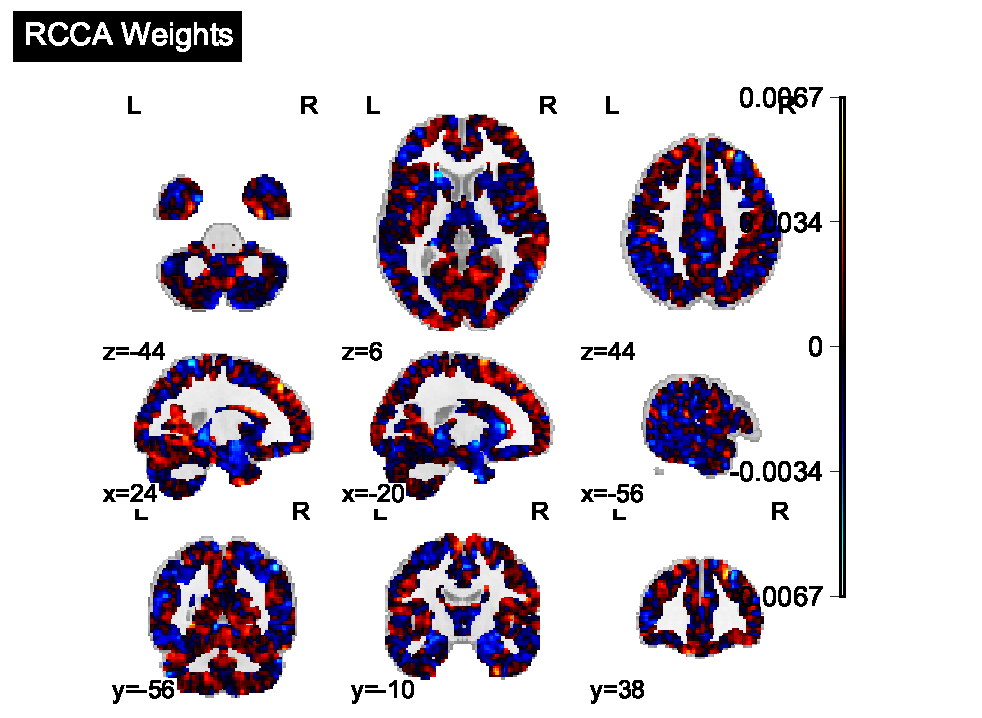
\includegraphics[width=0.45\linewidth]{figures/adni/RCCA brain weights mosaic}
    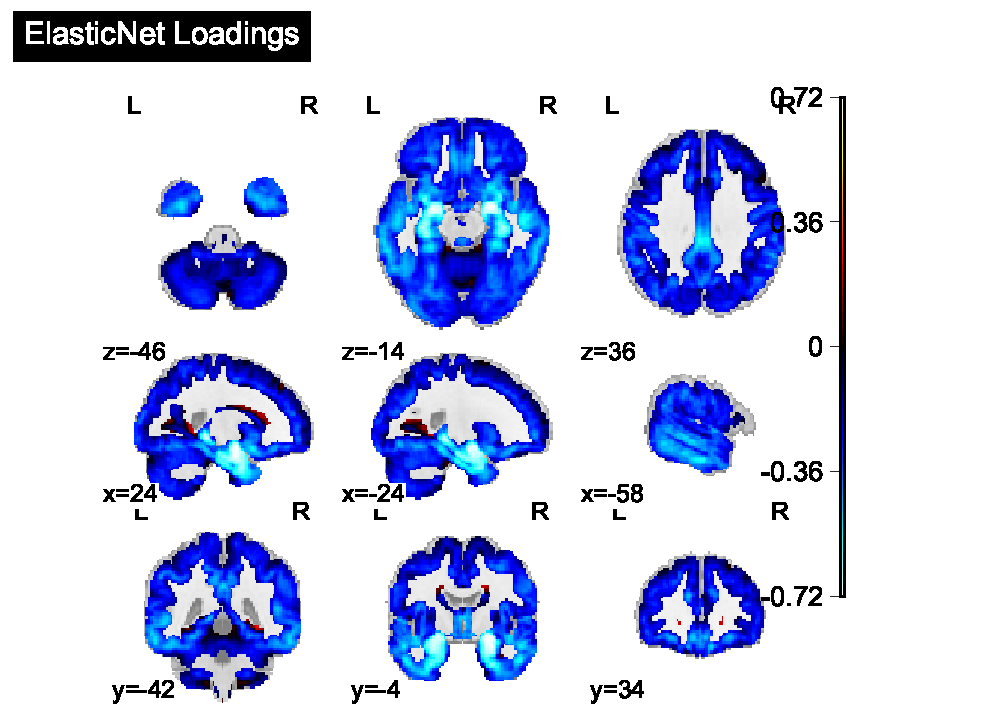
\includegraphics[width=0.45\linewidth]{figures/adni/ElasticNet brain loadings mosaic}
    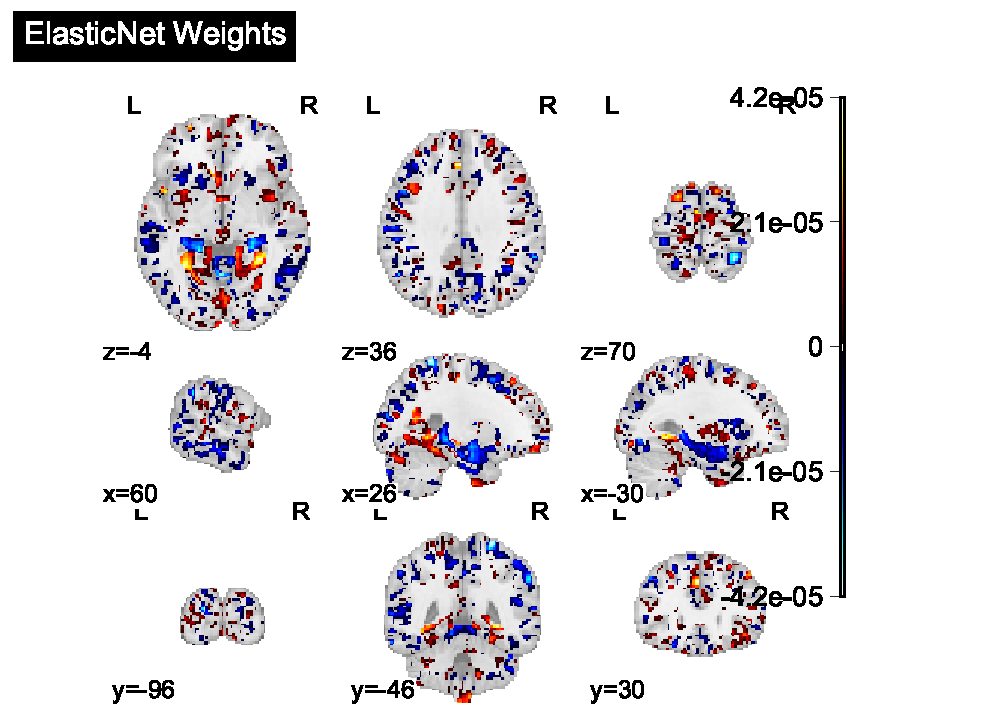
\includegraphics[width=0.45\linewidth]{figures/adni/ElasticNet brain weights mosaic}
    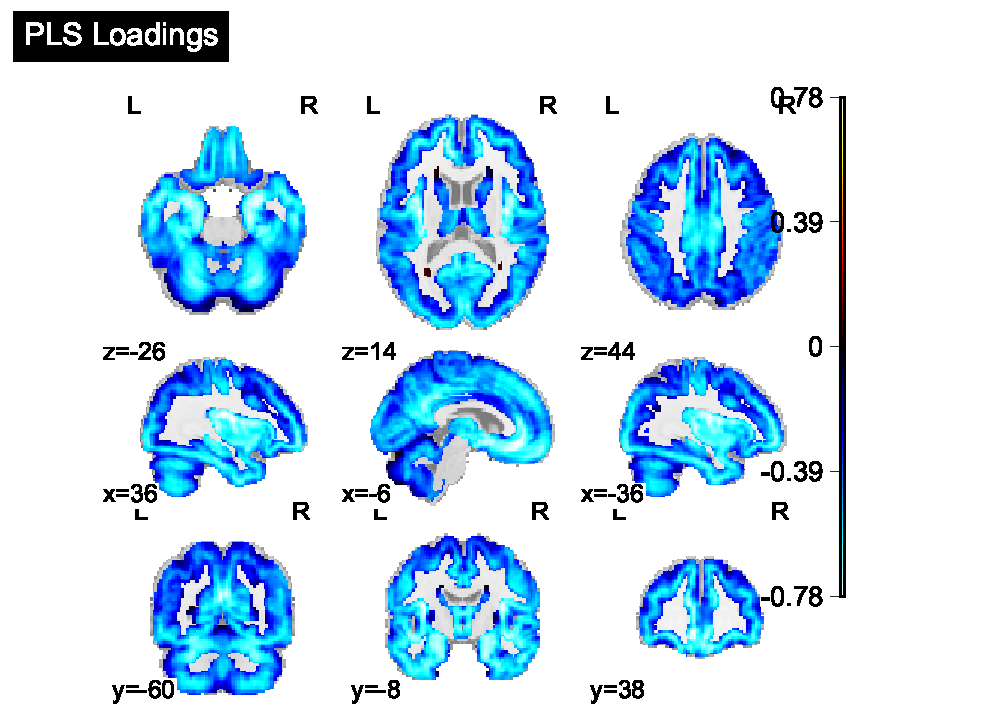
\includegraphics[width=0.45\linewidth]{figures/adni/PLS brain loadings mosaic}
    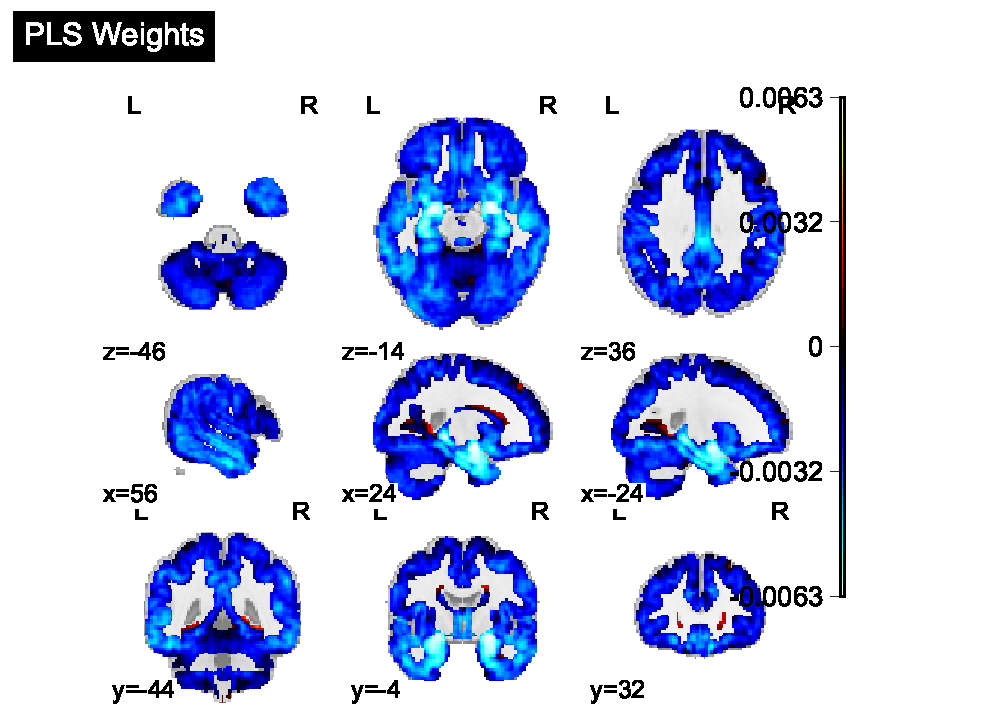
\includegraphics[width=0.45\linewidth]{figures/adni/PLS brain weights mosaic}
    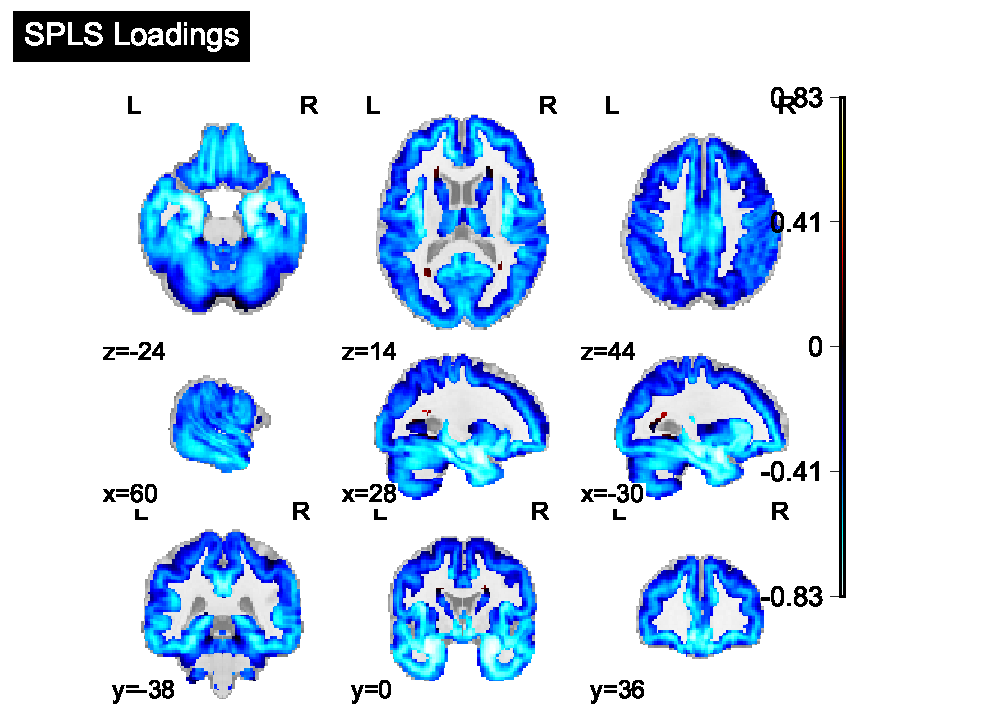
\includegraphics[width=0.45\linewidth]{figures/adni/SPLS brain loadings mosaic}
    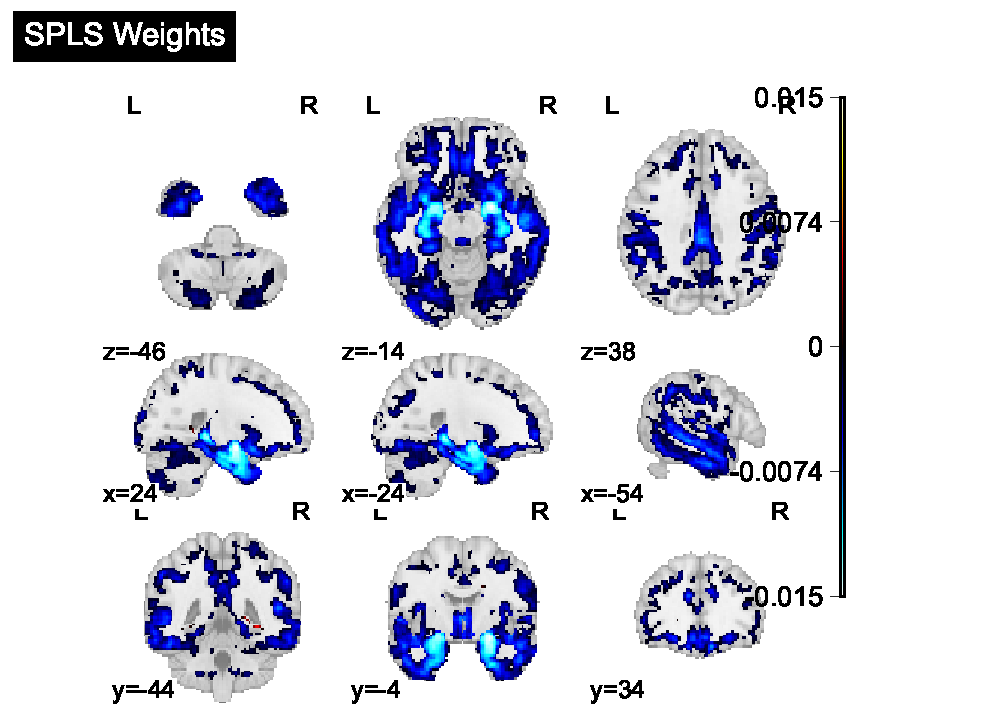
\includegraphics[width=0.45\linewidth]{figures/adni/SPLS brain weights mosaic}
    \caption{Statistical maps of brain structure \gls{loadings} and \gls{weights} for each model.}\label{fig:adni-brain}
\end{figure}